\documentclass{article}

\usepackage[romanian]{babel}
\usepackage{graphicx}

\graphicspath{ {../images/} }

\title{Tema 1 Inteligență Artificiala: Sokoban}
\author{Alexandru Sima (332CA)}

\begin{document}
\maketitle
\tableofcontents

\section{Beam search}

Am început prin a sorta starile in functie de distantele de la cutii la 
obiective, apoi de la jucator la cutii (pentru a nu avea egalitate intre starile
in care nu se muta o cutie). Nu s-a dovedit folositor nici macar pentru exemplul
din schelet, deoarece se impingea cutia in perete (mai aproape - d.p.d.v al 
distanței Manhattan - de obiectiv, apoi se bloca).
\begin{figure}[ht]
    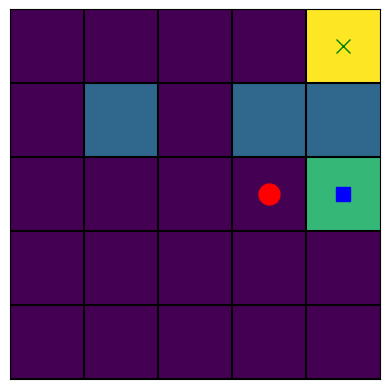
\includegraphics[scale=0.4]{a}
    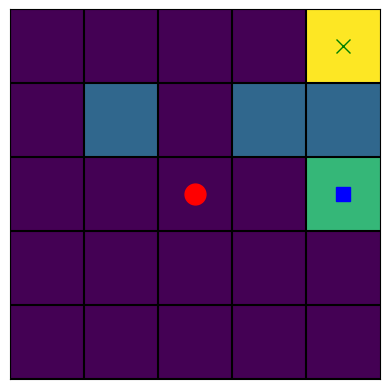
\includegraphics[scale=0.4]{b}
    \caption{Primul impas: Cutia nu poate fi adusă la țintă fără a fi 
    îndepărtată întâi de aceasta}
\end{figure}

O optimizare a evaluării stărilor a fost ca distanța cutiilor spre obiective să 
nu mai fie calculata folosind distanta Manhattan, ci prin cel mai scurt drum 
prin arenă de la cutie la o țintă. Cum țintele erau fixe, aceste distanțe se pot
precalcula pentru eficientizare. Această nouă versiune ajungea în continuare 
într-un impas, cand jucătorul trebuia sa se îndepărteze de o cutie pentru a o 
muta din alt unghi.
\begin{figure}[ht]
    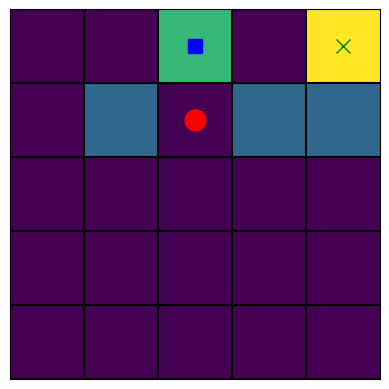
\includegraphics[scale=0.4]{a2}
    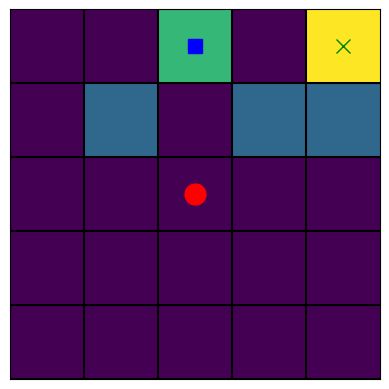
\includegraphics[scale=0.4]{b2}
    \caption{Al 2-lea impas: Cutia nu poate fi mutată fără ca jucătorul să se 
    îndepărteze de aceasta}
\end{figure}

\end{document}